\documentclass[a4paper,11pt]{article}
\usepackage[utf8]{inputenc}
\usepackage{geometry}
\usepackage{graphicx}
\usepackage{listings}
\usepackage{xcolor}
\usepackage{tikz}
\usetikzlibrary{shapes.geometric, arrows, positioning}

\geometry{left=2.5cm,right=2.5cm,top=2cm,bottom=2cm}

\definecolor{backcolour}{rgb}{0.95,0.95,0.92}
\definecolor{codegreen}{rgb}{0,0.6,0}
\definecolor{codeblue}{rgb}{0.1,0.1,0.6}

\lstdefinestyle{pythonstyle}{
    backgroundcolor=\color{backcolour},   
    commentstyle=\color{codegreen},
    keywordstyle=\color{codeblue}\bfseries,
    basicstyle=\ttfamily\small,
    breakatwhitespace=false,         
    breaklines=true,                 
    captionpos=b,                    
    keepspaces=true,                 
    numbers=left,                    
    numbersep=5pt,                  
    showspaces=false,                
    showstringspaces=false,
    showtabs=false,                  
    tabsize=2,
    frame=lines
}
\lstset{style=pythonstyle}

\title{\textbf{Practical Work 5: The Longest Path}}
\author{Group 16}
\date{\today}

\begin{document}

\maketitle

\section{Overview}
The goal of this practical work is to utilize the MapReduce programming model to identify the longest file path within a large dataset. This simulates a distributed operation where finding a global maximum requires aggregating local maximums from distributed nodes.

\section{Implementation Strategy}
We utilized Python's \textbf{multiprocessing} library to create a realistic simulation of a distributed environment.

\subsection{Why this approach?}
\begin{itemize}
    \item \textbf{Efficiency:} Instead of sending every single path to the Reducer (which would cause network congestion), each Mapper performs a "Local Reduce." It calculates the longest path within its assigned chunk and transmits only that single candidate to the Reducer.
    \item \textbf{Parallelism:} The dataset is split into chunks, and multiple worker processes scan these chunks simultaneously.
\end{itemize}

\section{System Architecture}

\subsection{Data Flow Diagram}
The figure below demonstrates how the system filters data. Unlike Word Count which expands data, Longest Path reduces data volume at every step.

\begin{figure}[h]
    \centering
    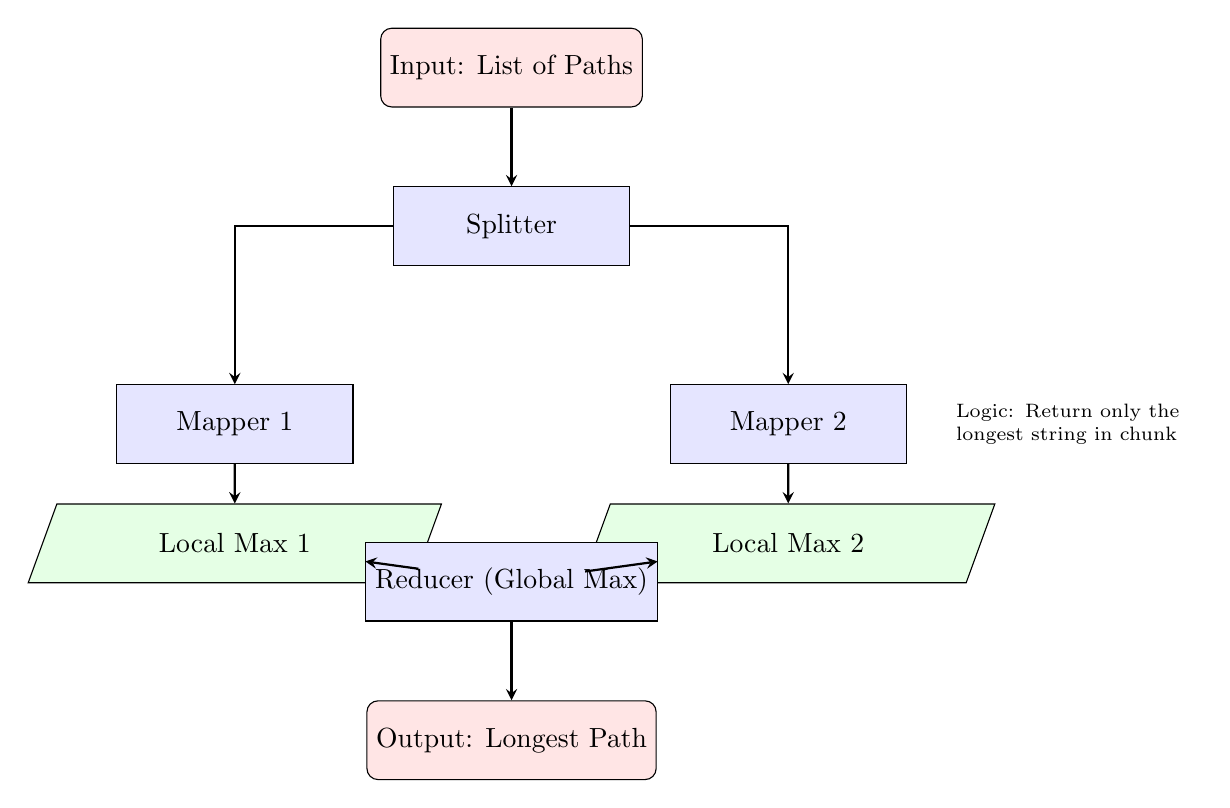
\begin{tikzpicture}[
        node distance=1.5cm,
        startstop/.style={rectangle, rounded corners, minimum width=2.5cm, minimum height=1cm, text centered, draw=black, fill=red!10},
        process/.style={rectangle, minimum width=3cm, minimum height=1cm, text centered, draw=black, fill=blue!10},
        decision/.style={trapezium, trapezium left angle=70, trapezium right angle=110, minimum width=2.5cm, minimum height=1cm, text centered, draw=black, fill=green!10},
        arrow/.style={thick,->,>=stealth}
    ]

    \node (input) [startstop] {Input: List of Paths};
    \node (split) [process, below=1cm of input] {Splitter};
    
    \node (map1) [process, below left=1.5cm and 0.5cm of split] {Mapper 1};
    \node (map2) [process, below right=1.5cm and 0.5cm of split] {Mapper 2};
    
    \node (out1) [decision, below=0.5cm of map1] {Local Max 1};
    \node (out2) [decision, below=0.5cm of map2] {Local Max 2};
    
    \node (reducer) [process, below=3.5cm of split] {Reducer (Global Max)};
    \node (final) [startstop, below=1cm of reducer] {Output: Longest Path};

    \draw [arrow] (input) -- (split);
    \draw [arrow] (split) -| (map1);
    \draw [arrow] (split) -| (map2);
    \draw [arrow] (map1) -- (out1);
    \draw [arrow] (map2) -- (out2);
    \draw [arrow] (out1) -- (reducer);
    \draw [arrow] (out2) -- (reducer);
    \draw [arrow] (reducer) -- (final);
    
    \node [right=0.5cm of map2, text width=3cm, font=\scriptsize] {Logic: Return only the longest string in chunk};

    \end{tikzpicture}
    \caption{MapReduce Data Flow for Longest Path}
    \label{fig:longestpath_flow}
\end{figure}

\subsection{Mapper Logic}
The mapper iterates through its assigned list of strings and keeps only the longest one.

\begin{lstlisting}[language=Python, caption=Mapper Function]
def map_worker(path_chunk):
    if not path_chunk:
        return None
    # Efficiently find the longest string in the list
    local_longest = max(path_chunk, key=len)
    return ("MAX", local_longest)
\end{lstlisting}

\subsection{Reducer Logic}
The reducer receives a list of "Local Maximums" from all mappers and selects the winner.

\begin{lstlisting}[language=Python, caption=Reducer Function]
def reduce_worker(item):
    key, paths = item
    # Compare local maximums to find global maximum
    global_longest = max(paths, key=len)
    return (key, global_longest)
\end{lstlisting}

\section{Roles and Responsibilities}
\begin{table}[h]
\centering
\begin{tabular}{|l|l|p{6cm}|}
\hline
\textbf{Member} & \textbf{Task} & \textbf{Details} \\ \hline
Member 1 & Driver Code & Implemented file reading, data splitting, and process pool management. \\ \hline
Member 2 & Map/Reduce Logic & Implemented the max-length logic and optimized the local-reduce strategy. \\ \hline
Member 3 & Documentation & Created the architecture diagram and compiled the LaTeX report. \\ \hline
\end{tabular}
\caption{Group Task Allocation}
\end{table}

\end{document}